\documentclass[aspectratio=169,10pt]{beamer}

\usetheme{Madrid}
\usecolortheme{seahorse}
\setbeamertemplate{navigation symbols}{}
\setbeamertemplate{caption}[numbered]

\usepackage[T1]{fontenc}
\usepackage[utf8]{inputenc}
\usepackage{booktabs}
\usepackage{graphicx}
\usepackage{listings}
\usepackage{array}
\usepackage{xcolor}

\graphicspath{{docs/report/}{report/}}

\definecolor{slrblue}{RGB}{38,84,124}
\definecolor{slrgreen}{RGB}{47,122,105}
\definecolor{slrgray}{RGB}{245,247,250}

\setbeamercolor{structure}{fg=slrblue}
\setbeamercolor{title}{fg=white,bg=slrblue}
\setbeamercolor{frametitle}{fg=white,bg=slrblue}
\setbeamercolor{block title}{fg=white,bg=slrgreen}
\setbeamercolor{block body}{bg=slrgray,fg=black}

\lstset{
  basicstyle=\ttfamily\small,
  columns=fullflexible,
  keepspaces=true,
  showstringspaces=false,
  breaklines=true,
  frame=single,
  backgroundcolor=\color{slrgray}
}

\title[Distributed MapReduce]{Distributed MapReduce on Lab Machines}
\subtitle{SLR Project P4}
\author{Project presentation}
\date{10-minute discussion}

\begin{document}

\begin{frame}
  \titlepage

  \vspace{-0.5em}
  \begin{block}{One-sentence summary}
    A custom Go MapReduce framework running on \texttt{*.enst.fr} workers — direct Common Crawl input, pluggable jobs, local-disk shuffle, fault-aware coordination, no root, no Docker.
  \end{block}
  \note{Timing: 20 seconds. No introduction needed beyond the block.}
\end{frame}

\begin{frame}{What We Built}
  \begin{itemize}
    \item Host discovery from \texttt{tp.telecom-paris.fr/ajax.php} — live JSON, canonical \texttt{.enst.fr} names, $2\times N$ pool for cold spares
    \item Go orchestrator: build worker binary, deploy, coordinate phases, merge results
    \item HTTP worker API: \texttt{/load} $\to$ \texttt{/map} $\to$ \texttt{/intermediate} $\to$ \texttt{/reduce} $\to$ \texttt{/result}
    \item Four pluggable jobs sharing the same framework: \texttt{wordcount}, \texttt{langdetect}, \texttt{domainpop}, \texttt{docdensity}
    \item 89 Go tests; reference wordcount matched exactly against sequential implementation
  \end{itemize}
  \note{Timing: 45 seconds. The core distributed computation is real — workers map, write buckets, fetch from peers, reduce.}
\end{frame}

\begin{frame}{Key Design Choices}
  \begin{columns}[T,onlytextwidth]
    \begin{column}{0.48\textwidth}
      \textbf{Storage: everything avoids NFS}
      \begin{itemize}
        \item Input: streamed directly from \texttt{data.commoncrawl.org} (Amazon S3) — \texttt{/cal/commoncrawl} never read
        \item Intermediate bucket files: \texttt{os.MkdirTemp} $\to$ \texttt{/tmp} on each worker
        \item Worker binary: SCPed to \texttt{/tmp/mr-worker}, not \texttt{\$HOME}
        \item Final output: written locally on the orchestrator
      \end{itemize}
    \end{column}
    \begin{column}{0.48\textwidth}
      \textbf{Deployment: $N$ SCP to \texttt{/tmp}}
      \begin{itemize}
        \item Binary cross-compiled locally (\texttt{GOOS=linux GOARCH=amd64})
        \item $N$ SCPs directly to \texttt{/tmp} (vs.\ rubric's 1 SCP to NFS home)
        \item Trade-off: avoids NFS entirely; acceptable for $N \leq 20$
        \item SSH multiplexing (\texttt{ControlMaster}): SCP and start share one TCP connection
        \item \texttt{BatchMode=yes}, \texttt{StrictHostKeyChecking=no}, \texttt{ConnectTimeout=10}
      \end{itemize}
    \end{column}
  \end{columns}
  \note{Timing: 1 minute. This slide directly answers the NFS/deployment exam questions. The key message: every hot-path write goes to local /tmp; the NFS is only touched for the final small result file if the user chooses a home path.}
\end{frame}

\begin{frame}{Protocol and Dataflow}
  \begin{columns}[T,onlytextwidth]
    \begin{column}{0.50\textwidth}
      \begin{enumerate}
        \item \textbf{Load} — Common Crawl URLs via \texttt{POST /load}; workers download WET files to \texttt{/tmp}
        \item \textbf{Map} — each worker writes $N$ bucket files on local disk (\texttt{/tmp})
        \item \textbf{Shuffle+Reduce} — reducer $i$ pulls bucket $i$ from every peer via \texttt{GET /intermediate} (P2P, no orchestrator)
        \item \textbf{Collect} — orchestrator fetches \texttt{/result}, merges, sorts, writes output
      \end{enumerate}
    \end{column}
    \begin{column}{0.46\textwidth}
      \begin{block}{Partitioning}
        \texttt{FNV-32a(key) \% N}\\[0.4em]
        All values for the same key always route to the same reducer. $N$ stays \textbf{fixed} for the job — changing it mid-run would split the value list across two reducers.
      \end{block}
      \begin{block}{Bootstrap}
        Workers start independently. Peers are discovered only when the orchestrator sends \texttt{POST /reduce \{peers:[...]\}}.
      \end{block}
    \end{column}
  \end{columns}
  \note{Timing: 1 minute 20 seconds. Emphasise P2P shuffle — no data flows through the orchestrator. The orchestrator is a coordinator, not a data plane.}
\end{frame}

\begin{frame}{Fault Tolerance}
  \begin{columns}[T,onlytextwidth]
    \begin{column}{0.50\textwidth}
      \textbf{Detection}
      \begin{itemize}
        \item Health watcher polls \texttt{GET /health} every 5\,s
        \item Host declared dead after \textbf{2 consecutive failures}
      \end{itemize}
      \textbf{Recovery}
      \begin{itemize}
        \item Slot $\to$ spare host; slot state reset to \texttt{pending}
        \item Prerequisites replayed: \texttt{load} $\to$ \texttt{map} $\to$ \texttt{reduce}
        \item \textbf{Epoch} incremented: any reduce at old epoch is rewound and re-run (peer set changed)
      \end{itemize}
    \end{column}
    \begin{column}{0.46\textwidth}
      \begin{block}{Atomic writes}
        WET downloads: \texttt{CreateTemp} + \texttt{os.Rename} (ok)\\
        Binary deploy: \texttt{mv} on same filesystem (ok)\\
        Final output: direct write (known gap)
      \end{block}
      \begin{block}{Known gaps}
        No speculative execution for stragglers.\\
        Orchestrator crash $\Rightarrow$ job must restart (workers survive via \texttt{nohup}).
      \end{block}
    \end{column}
  \end{columns}
  \note{Timing: 55 seconds. The epoch mechanism is the most interesting part — it guarantees that a reduce whose peer set changed is never silently accepted.}
\end{frame}

\begin{frame}{Use Cases Beyond Wordcount}
  \begin{itemize}
    \item \textbf{langdetect} — stop-word scoring per line (EN/FR/DE/ES/IT); WARC headers skipped; result: language share across the crawl. \textit{Common Crawl is $\approx$60\,\% English.}
    \item \textbf{domainpop} — reads \texttt{WARC-Target-URI:} header per WET record; counts pages per domain; result: global domain popularity ranking (\textit{youtube.com, wikipedia.org, doi.org} top-ranked). Quality signal: unexpectedly high-ranked spam domains flag filtering needs.
    \item \textbf{docdensity} — counts chars, alphanumeric ratio, and line-length histogram per content line; result: $\approx$77\,\% alphanumeric, most lines $<$80 chars, very long lines $=$ minified JS/CSS.
  \end{itemize}
  \begin{block}{Why Common Crawl matters}
    One of the primary training data sources for GPT, LLaMA, Mistral and most modern LLMs. These jobs are the kind of analysis that precedes any large-scale dataset curation.
  \end{block}
  \note{Timing: 45 seconds. Stress that all four jobs reuse the same deploy/shuffle/reduce/collect path. Only the map and reduce functions differ.}
\end{frame}

\begin{frame}{Measurements and Amdahl's Law}
  \begin{columns}[T,onlytextwidth]
    \begin{column}{0.57\textwidth}
      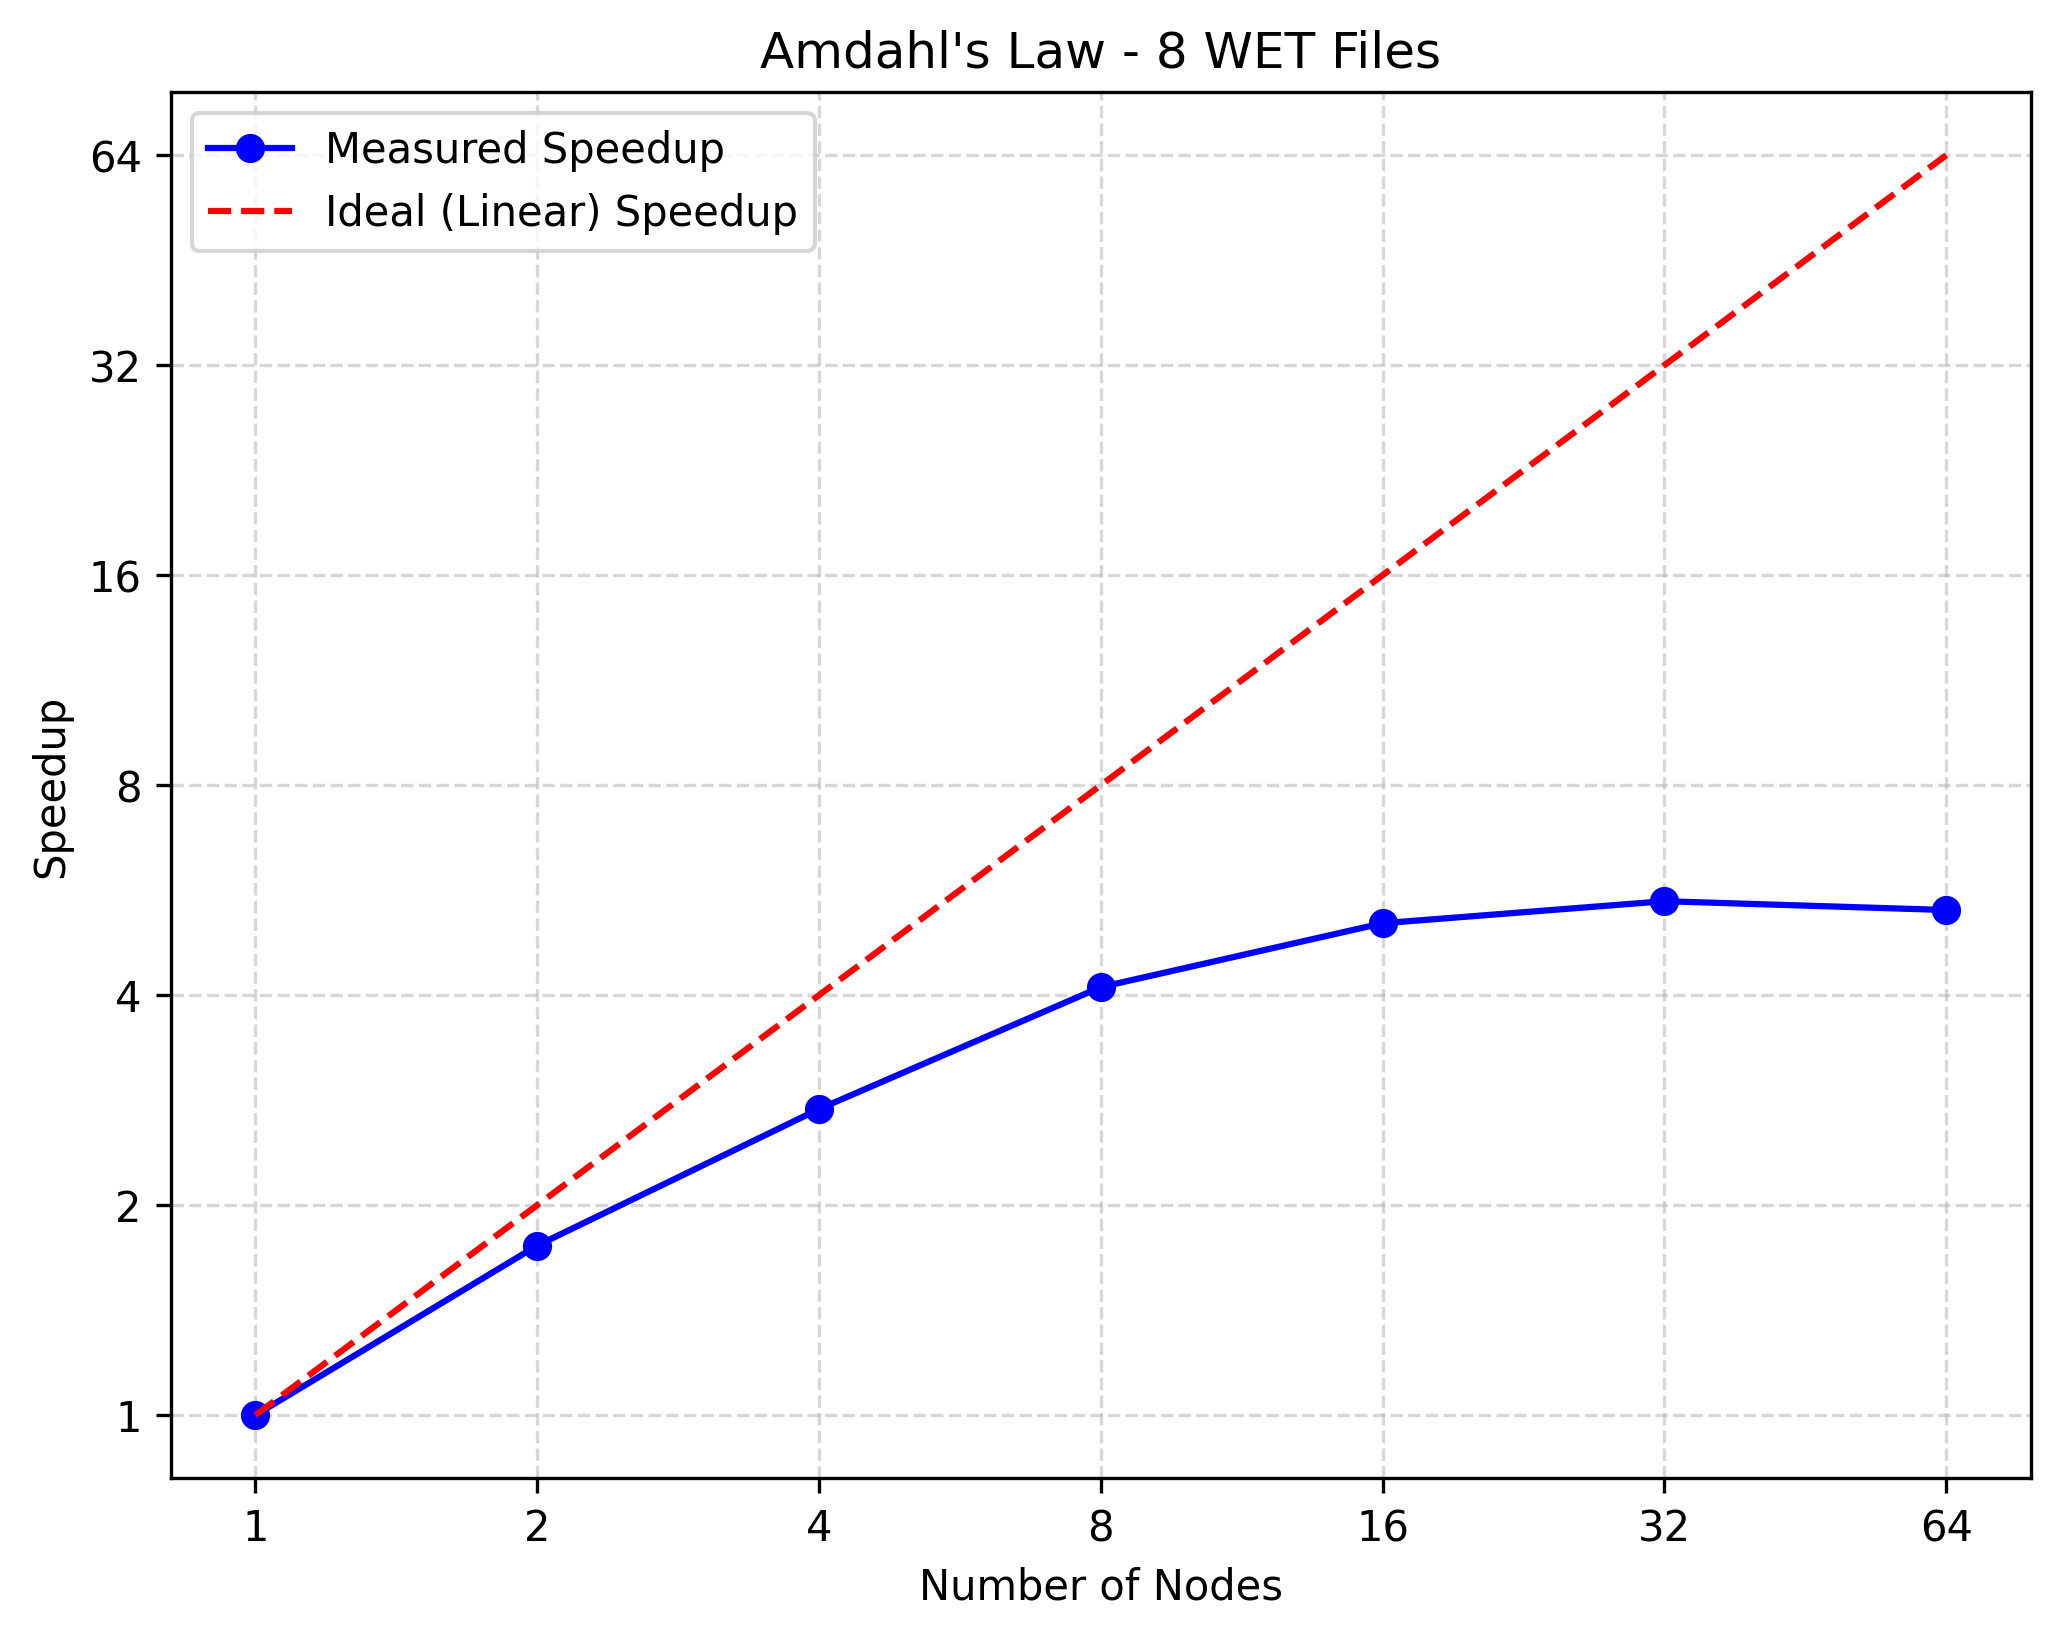
\includegraphics[width=\linewidth]{amdahl_8.png}
    \end{column}
    \begin{column}{0.4\textwidth}
      \begin{itemize}
        \item Same 8 WET files at every point (correct methodology)
        \item \texttt{1 node}: 206.95\,s $\Rightarrow$ baseline
        \item \texttt{16 nodes}: 40.80\,s, speedup 5.07
        \item \texttt{64 nodes}: 39.06\,s — \emph{regression}
      \end{itemize}
      \begin{block}{Serial fraction}
        Plateau $S\!\approx\!5.45$ $\Rightarrow$ $f\!\approx\!18\%$ serial.\\
        Source: orchestrator collect phase (sequential merge of $N$ results) and $N\!\times\!(N\!-\!1)$ HTTP connections at 64 nodes.
      \end{block}
    \end{column}
  \end{columns}
  \note{Timing: 1 minute 15 seconds. f=18\% means 82\% of the work is parallelisable. The collect phase grows with N and becomes the ceiling.}
\end{frame}

\begin{frame}{Three-Way Comparison}
  \begin{table}
    \small
    \begin{tabular}{l p{0.26\linewidth} p{0.26\linewidth} p{0.26\linewidth}}
      \toprule
       & \textbf{Our MapReduce} & \textbf{Hadoop} & \textbf{Kafka Streams} \\
      \midrule
      Model & Batch, 1 stage & Batch, multi-stage & Stream, unbounded \\
      Storage & \texttt{/tmp}, no replication & HDFS 3$\times$ replication & Replicated broker log \\
      Data locality & No — HTTP pull & Yes — run where data lives & Broker partitions \\
      Stragglers & Not handled & Speculative execution & N/A \\
      8-node wordcount & 0.27\,s & not run & 10.1\,s \\
      \bottomrule
    \end{tabular}
  \end{table}
  \begin{block}{Biggest gaps vs.\ Hadoop}
    (1) HDFS data locality — we transfer all input at load time.
    (2) Speculative execution — one slow node blocks the whole phase.
  \end{block}
  \note{Timing: 55 seconds. Kafka difference is model-level (stream vs batch). Hadoop difference is engineering-level (production data locality + scheduling we did not build).}
\end{frame}

\begin{frame}[fragile]{What's Missing + Demo}
  \begin{columns}[T,onlytextwidth]
    \begin{column}{0.44\textwidth}
      \textbf{Real remaining gaps}
      \begin{itemize}
        \item Atomic final output write (temp+rename)
        \item Speculative execution for stragglers
        \item Port collision preflight check
        \item Multi-chunk scheduling in local-file mode
        \item Cross-login validation
      \end{itemize}
    \end{column}
    \begin{column}{0.52\textwidth}
      \begin{block}{Live demo}
\begin{lstlisting}[basicstyle=\ttfamily\scriptsize]
cd scripts && go test ./...
./mapreduce.sh \
  -job scripts/jobs/wordcount \
  -input test_input.txt \
  -n 4 -output result.txt
./run_all_commoncrawl_jobs.sh \
  -crawl CC-MAIN-2026-21 \
  -files-limit 1 -n 4
\end{lstlisting}
      \end{block}
      \begin{block}{Backup if machines are unstable}
        {\small Passed tests, checked-in wordcount output (24M unique words), Amdahl plot, timing CSVs}
      \end{block}
    \end{column}
  \end{columns}
  \note{Timing: 1 minute 15 seconds. Be calm about gaps — the protocol, jobs, and recovery all work and are tested. The gaps are operational hardening.}
\end{frame}

\end{document}
